
%==================================================
%%%%%%%%%%%%%%%%%%%%%%%%%%%%%%%%%%%%%%%%%%%%%%%%%%%%
\chapter{Gestion du projet : Analyse et Planification}

\section{Introduction}
Nous allons, dans ce chapitre, approfondir les besoins qui motivent le développement du système Smart Focus. C’est une étape clé pour s’assurer que la solution finale réponde aux attentes des utilisateurs et aux contraintes techniques identifiées.

En faisant partie de l’équipe projet et en assurant les différentes missions qui nous ont été assignées, nous avons pris une part active à cette phase d’analyse. Nous verrons tout d’abord comment les besoins ont été collectés, puis analysés et priorisés. Nous présenterons ensuite les acteurs du système, les diagrammes de cas d’utilisation ainsi que l’architecture globale adoptée. Enfin, nous allons rentrer dans le détail de la planification des sprints. Cette démarche vise à établir une base solide pour la suite du projet, en alignant clairement les objectifs fonctionnels et techniques.

Cette démarche vise à poser les bases du projet, en alignant clairement les objectifs fonctionnels et techniques sur les attentes réelles des utilisateurs.
%%%%%%%%%%%%%%%%%%%%%%%%%%%%%%%%%%%%%%%%%%%%%%%%%%%%
% RECUEIL DES BESOINS
%%%%%%%%%%%%%%%%%%%%%%%%%%%%%%%%%%%%%%%%%%%%%%%%%%%%
\section{Recueil des besoins}

La collecte des besoins constitue une étape essentielle dans la conception du système \textit{SmartFocus}. Elle permet de comprendre les attentes des utilisateurs, d’identifier les fonctionnalités nécessaires et de définir les contraintes du projet.

Cette démarche vise à poser les bases d’une suite solide du projet, en alignant clairement les objectifs fonctionnels et techniques avec les attentes réelles. Pour obtenir une vision claire et réaliste, plusieurs approches complémentaires ont été adoptées.
% IDENTIFICATION DES ACTEURS
%%%%%%%%%%%%%%%%%%%%%%%%%%%%%%%%%%%%%%%%%%%%%%%%%%%%
\subsection{Identification des acteurs}
Le système \textit{Smart Focus} met en jeu plusieurs acteurs, qu’ils soient principaux ou secondaires. Le tableau suivant présente de manière synthétique le rôle de chacun au sein du système.


\begin{table}[H]
\centering
\renewcommand{\arraystretch}{1.5}
\setlength{\tabcolsep}{8pt}

\begin{tabularx}{\textwidth}{|>{\raggedright\arraybackslash}p{4cm}|c|>{\raggedright\arraybackslash}X|}
\hline
\textbf{Acteur} & \textbf{Type} & \textbf{Description} \\
\hline

Utilisateur 
& Principal 
& Étudiant, professionnel ou enseignant utilisant le système pour suivre sa concentration, gérer ses sessions et consulter les informations fournies. \\
\hline

Service d’intelligence artificielle externe 
& Secondaire 
& Service externe accessible via API, utilisé pour analyser les données, générer des recommandations et fournir des fonctionnalités intelligentes (chatbot, assistance). \\
\hline

\end{tabularx}

\caption{Identification des acteurs du système}
\label{tab:acteurs}

\end{table}
%\subsection{Identification des besoins}

%En se basant sur les méthodes de recueil décrites ci-dessus, il a été possible d’identifier plusieurs besoins clés pour le projet \textit{Smart Focus}. Ces besoins traduisent à la fois les attentes des utilisateurs en matière de fonctionnalités et les contraintes techniques à respecter.

%\vspace{0.5em}
%\begin{table}[H]
 %   \centering
  %\begin{tabular}{|p{5.5cm}|p{8.5cm}|}
   %     \hline
      %  \textbf{Catégorie} & \textbf{Description} \\ \hline
      %  Détection de la concentration & Analyse en temps réel de la posture, de la fatigue et des distractions via la vision par ordinateur pour calculer un score de concentration. \\ \hline
       % Planification intelligente & Génération automatique de sessions d'étude adaptées au profil de l'utilisateur, à son sommeil et à ses examens à venir, en exploitant l'\ac{IA}. \\ \hline
      %  Assistance pédagogique & Chatbot \ac{RAG} permettant de poser des questions sur ses cours (PDF), de générer des quiz QCM et des flashcards avec répétition espacée. \\ \hline
      %  Suivi du sommeil & Enregistrement et analyse de la qualité du sommeil, avec adaptation automatique de la charge de travail du lendemain. \\ \hline
     %   Feedback intelligent & Retours visuels (LEDs, écran TFT), sonores et via notifications mobiles pour alerter l'utilisateur en cas de baisse de concentration ou de mauvaise posture. \\ \hline
     %   Interface mobile ergonomique & Application Flutter intuitive offrant dashboard, statistiques, gestion des sessions et accès à toutes les fonctionnalités du système. \\ \hline
 %   \end{tabular}
 %   \caption{Synthèse des besoins identifiés}
 %   \label{tab:besoins_identifies}
%\end{table}


%%%%%%%%%%%%%%%%%%%%%%%%%%%%%%%%%%%%%%%%%%%%%%%%%%%%
% ANALYSE DES BESOINS
%%%%%%%%%%%%%%%%%%%%%%%%%%%%%%%%%%%%%%%%%%%%%%%%%%%%
\subsection{Identification des besoins}

Pour mieux structurer les exigences du projet \textit{Smart Focus}, les besoins identifiés ont été classés selon leur nature et leur rôle dans le fonctionnement global du système. Cette classification facilite la compréhension des priorités et des contraintes à prendre en compte.

\vspace{0.5em}
\begin{itemize}
    \item \textbf{Besoins fonctionnels} :
    \begin{itemize}
        \item Capturer et analyser les données visuelles afin d'évaluer la posture, la fatigue et le niveau de concentration de l'utilisateur en temps réel.
        \item Détecter les situations de distraction et générer des alertes adaptées.
        \item Calculer un score de concentration dynamique basé sur plusieurs indicateurs comportementaux.
        \item Gérer des sessions de travail intelligentes, incluant le démarrage, le suivi et l'historique.
        \item Proposer un système de planification adaptatif permettant d'organiser les sessions en fonction de l'état de l'utilisateur (fatigue, concentration, sommeil) et de ses examens.
        \item Intégrer un assistant pédagogique basé sur un chatbot \ac{RAG} permettant d'exploiter des documents (PDF et CSV), de répondre aux questions, de générer des quiz et des flashcards.
        \item Offrir un système de suivi du sommeil permettant d'évaluer sa qualité et d'influencer l'organisation des activités.
        \item Fournir un accompagnement via un agent vocal intelligent capable d'interagir avec l'utilisateur et de proposer des recommandations.
        \item Afficher les données et statistiques à travers une application mobile.
        \item Assurer la synchronisation des données entre les différents composants du système (boîtier \ac{IoT}, backend, application).
    \end{itemize}

    \item \textbf{Besoins non fonctionnels} :
    \begin{itemize}
        \item \textbf{Performance :} Traitement rapide des données garantissant un fonctionnement en temps réel.
        \item \textbf{Précision :} Analyses IA fiables et cohérentes.
        \item \textbf{Ergonomie :} Interface simple, intuitive et adaptée à une utilisation quotidienne.
        \item \textbf{Disponibilité :} Fonctionnement maintenu même en cas de perte temporaire de connexion.
        \item \textbf{Scalabilité :} Architecture permettant l'ajout de nouvelles fonctionnalités.
        \item \textbf{Sécurité :} Protection des données de l'utilisateur (\ac{JWT}, bcrypt).
        \item \textbf{Compatibilité :} Fonctionnement sur plateforme embarquée et accès via application mobile.
        \item \textbf{Maintenabilité :} Code structuré facilitant les mises à jour et améliorations.
    \end{itemize}

    \item \textbf{Contraintes} :
    \begin{itemize}
        \item Ressources matérielles limitées de Raspberry (mémoire, puissance de calcul).
        \item Dépendance à un service \ac{LLM} externe (Google Gemini) nécessitant une connexion Internet.
        \item Séparation des responsabilités entre deux membres de l'équipe (hardware / logiciel).
        \item Compatibilité avec les technologies retenues (FastAPI, Flutter, PostgreSQL, ChromaDB).
    \end{itemize}
\end{itemize}
\vspace{1em}

\noindent\colorbox{gray!15}{%
    \parbox{\dimexpr\linewidth-2\fboxsep}{%
        \small
        \textbf{Résumé :} Cette classification permet de mieux cibler les efforts de développement en mettant en lumière les aspects essentiels à couvrir pour assurer la réussite du projet.
    }%
}

\subsection{Priorisation des besoins}

Afin d'assurer le progrès efficace du projet \textit{Smart Focus}, il est primordial de classer les besoins selon leur influence sur les utilisateurs et leur viabilité technique. Cette phase permet de focaliser les efforts sur les fonctionnalités qui sont les plus cruciales.

\vspace{0.5em}
\begin{table}[H]
    \centering
    \renewcommand{\arraystretch}{1.3}
    
    \begin{tabular}{|p{5cm}|p{6.5cm}|c|}
        \hline
        \textbf{Besoin} & \textbf{Justification} & \textbf{Priorité} \\ \hline
        
        Authentification et gestion de profil 
        & Nécessaire pour la gestion des utilisateurs et la persistance des données 
        & Haute \\ \hline
        
        Détection de la concentration (score focus) 
        & Cœur du système basé sur la vision par ordinateur et le hardware 
        & Haute \\ \hline
        
        Chatbot \ac{RAG} (upload, chat, quiz, flashcards) 
        & Apporte une forte valeur ajoutée pédagogique et personnalisation via l’IA 
        & Haute \\ \hline
        
        Planification intelligente 
        & Permet d’adapter les sessions en fonction des données utilisateur et du niveau de fatigue 
        & Haute \\ \hline
        
        Dashboard et statistiques 
        & Permet l’analyse des performances et l’amélioration continue de l’utilisateur 
        & Moyenne \\ \hline
        
        Posture et feedback ergonomique 
        & Améliore l’expérience utilisateur via des recommandations physiques basées sur la vision 
        & Moyenne \\ \hline
        
        Suivi du sommeil et alarme 
        & Fonction complémentaire influençant indirectement la performance de l’utilisateur 
        & Basse \\ \hline
        
        Agent vocal intelligent 
        & Fonctionnalité avancée non essentielle, ajoutée en phase finale si possible 
        & Basse \\ \hline
        
    \end{tabular}

    \caption{Priorisation des besoins}
    \label{tab:priorisation_besoins}
\end{table}

\vspace{1em}
\noindent\colorbox{gray!15}{%
    \parbox{\dimexpr\linewidth-2\fboxsep}{%
        \textbf{Conclusion :} On a accordé la priorité aux besoins relatifs à l’authentification, à l’assistance pédagogique et à la planification intelligente, afin de poser une base solide pour le système tout en prévoyant une intégration progressive des fonctionnalités dépendant du hardware.
    }%
}

%%%%%%%%%%%%%%%%%%%%%%%%%%%%%%%%%%%%%%%%%%%%%%%%%%%%
% MODÉLISATION — CAS D'UTILISATION
%%%%%%%%%%%%%%%%%%%%%%%%%%%%%%%%%%%%%%%%%%%%%%%%%%%%
\section{Modélisation des besoins}

\subsection{Diagramme de cas d'utilisation global}
Le diagramme suivant, présente la liste de tous les cas d'utilisation du système Smart Focus, classés par module fonctionnel. Le système comporte 46 cas d’usage organisés en 9 modules.
\begin{figure}[htbp]
    \centering
    \includegraphics[width=1\textwidth]{images/UCDiagram.png}
    \caption{Diagramme de cas d'utilisation global}
    \label{fig:uml_global}
\end{figure}


\section{Planification du projet}
\subsection{Backlog du produit}
{\singlespacing
\begin{table}[H]
\centering
\small
\renewcommand{\arraystretch}{1.2}
\setlength{\tabcolsep}{5pt}

\begin{tabularx}{\textwidth}{|c|p{3cm}|X|c|c|}
\hline
\textbf{ID} & \textbf{Fonctionnalité} & \textbf{User Story} & \textbf{Priorité} & \textbf{ID} \\
\hline

US1 & Authentification 
& En tant qu’utilisateur, je veux créer un compte et me connecter afin d’accéder à mes données personnelles. 
& Haute & 1 \\ \hline

US2 & Démarrage session 
& En tant qu’utilisateur, je veux démarrer une session de travail afin de suivre mon niveau de concentration. 
& Haute & 2 \\ \hline

US3 & Capture vidéo (Raspberry Pi) 
& En tant que système, je veux capturer les images en temps réel afin d’analyser le comportement de l’utilisateur. 
& Haute & 3 \\ \hline

US4 & Détection de concentration 
& En tant que système, je veux analyser les images pour calculer un score de concentration. 
& Haute & 4 \\ \hline

US5 & Détection fatigue et posture 
& En tant que système, je veux détecter la fatigue et la posture afin d’évaluer l’état de l’utilisateur. 
& Haute & 5 \\ \hline

US6 & Enregistrement des métriques 
& En tant que système, je veux stocker les données de session afin de permettre leur exploitation. 
& Haute & 6 \\ \hline

US7 & Génération d’alertes 
& En tant que système, je veux déclencher des alertes lorsque la fatigue est élevée afin d’améliorer la concentration. 
& Haute & 7 \\ \hline

US8 & Affichage temps réel 
& En tant qu’utilisateur, je veux visualiser mes scores en temps réel sur l’application mobile. 
& Haute & 8 \\ \hline

US9 & Chatbot intelligent (RAG) 
& En tant qu’utilisateur, je veux interagir avec un chatbot pour poser des questions et réviser mes cours. 
& Haute & 9 \\ \hline

US10 & Import de documents 
& En tant qu’utilisateur, je veux importer mes cours afin qu’ils soient utilisés par le chatbot. 
& Haute & 10 \\ \hline

US11 & Génération de quiz/flashcards 
& En tant qu’utilisateur, je veux générer des quiz pour tester mes connaissances. 
& Moyenne & 11 \\ \hline

US12 & Planification intelligente 
& En tant qu’utilisateur, je veux obtenir un planning adapté à mon niveau de fatigue et mes performances. 
& Haute & 12 \\ \hline

US13 & Dashboard et statistiques 
& En tant qu’utilisateur, je veux visualiser mes performances pour suivre mon évolution. 
& Moyenne & 13 \\ \hline

US14 & Feedback ergonomique 
& En tant qu’utilisateur, je veux recevoir des recommandations sur ma posture. 
& Moyenne & 14 \\ \hline

US15 & Suivi du sommeil 
& En tant qu’utilisateur, je veux suivre mon sommeil afin d’améliorer mes sessions de travail. 
& Basse & 15 \\ \hline

US16 & Agent vocal 
& En tant qu’utilisateur, je veux interagir avec le système via la voix. 
& Basse & 16 \\ \hline

\end{tabularx}

\caption{Backlog du produit}
\label{tab:backlog}
\end{table}
}
%%%%%%%%%%%%%%%%%%%%%%%%%%%%%%%%%%%%%%%%%%%%%%%%%%%%%%%%%%%%%%%%%%%%%%%%%%%%%%%%%%%%%%%%%%%%%%%%%%%%%%%%%%%%%%%%%%%%%%%%%%%%%%%%%%


\subsection{Planification des sprints}

Le développement du projet a été organisé en quatre sprints successifs, chacun couvrant une période d’environ un mois. Cette planification a été définie de manière progressive afin d’assurer un équilibre entre les différentes composantes du système, notamment l’application mobile, les modules intelligents et la vision par ordinateur.
{\singlespacing
\begin{table}[H]
\centering
\small
\renewcommand{\arraystretch}{1.2}
\setlength{\tabcolsep}{5pt}

\begin{tabularx}{\textwidth}{|c|p{3.8cm}|X|c|}
\hline
\textbf{Sprint} & \textbf{Intitulé} & \textbf{Description} & \textbf{Durée} \\
\hline

Sprint 1 & 
Authentification et interfaces de base & 
Développement du module d’authentification permettant l’inscription, la connexion et la gestion du profil utilisateur côté backend et application mobile. Mise en place des interfaces principales de l’application (tableau de bord, statistiques, sommeil, paramètres) ainsi que de la navigation entre les écrans. &
20 jours \\ \hline

Sprint 2 & 
Surveillance intelligente de la concentration (Vision + Score) & 
Implémentation du module de vision par ordinateur permettant l’analyse en temps réel de l’état de l’utilisateur à partir du flux vidéo. Détection de la fatigue, des distractions et de la posture via des techniques d’intelligence artificielle, puis calcul d’un score global de concentration transmis au backend. &
40 jours \\ \hline

Sprint 3 & 
Planning intelligent et assistant d’apprentissage & 
Développement du système de planning intelligent basé sur l’intelligence artificielle pour la génération automatique des sessions d’étude. Intégration du chatbot RAG permettant l’interrogation de documents PDF, ainsi que la génération automatique de quiz et de flashcards avec révision espacée (SM-2). Connexion des interfaces mobiles aux données dynamiques du backend. &
30 jours \\ \hline

Sprint 4 & 
Système IoT et alertes intelligentes & 
Intégration du dispositif matériel de monitoring permettant la capture continue des données utilisateur via caméra et capteurs. Mise en place du suivi temps réel dans l’application mobile ainsi que du système d’alertes intelligentes basé sur le niveau de concentration et les données de sommeil afin d’adapter le comportement du système et le planning de travail. &
30 jours \\ \hline

\end{tabularx}

\caption{Planification des sprints du projet}
\label{tab:sprints_final}
\end{table}
}
%==================================================
\section{Diagramme de Gantt}

\begin{figure}[H]
\centering
\includegraphics[width=\textwidth]{images/gantt.png}
\caption{Diagramme de Gantt}
\end{figure}
%==================================================
\section{Environnement de travail}

\subsection{Choix des technologies}

Le développement du système \textit{Smart Focus} repose sur un ensemble de technologies modernes permettant de garantir performance, modularité et évolutivité. Les technologies retenues sont présentées ci-dessous, regroupées par catégorie.

\subsubsection{Langages de programmation}

\begin{itemize}

\item \textbf{Python :} Langage de programmation largement utilisé dans le développement web, l'intelligence artificielle et le traitement d'images. Dans notre projet, Python est utilisé pour développer le backend avec FastAPI, le pipeline de vision par ordinateur pour l'analyse en temps réel via caméra, ainsi que les modules d'intelligence artificielle .

\begin{figure}[H]
    \centering
    \includegraphics[width=0.15\textwidth]{images/pythonLogo.png}
    \caption{Logo Python}
\end{figure}

\item \textbf{Dart :} Langage de programmation développé par Google, optimisé pour la création d'interfaces utilisateur performantes et multiplateformes. Dans notre projet, Dart est le langage utilisé avec le framework Flutter pour développer l'application mobile Smart Focus .

\begin{figure}[H]
    \centering
    \includegraphics[width=0.3\textwidth]{images/dart.jpg}
    \caption{Logo Dart}
\end{figure}

\end{itemize}

\subsubsection{Frameworks et bibliothèques}

\begin{itemize}

\item \textbf{FastAPI :} Framework Python moderne conçu pour la création d'API REST performantes avec documentation automatique. Dans notre projet, FastAPI gère l'ensemble des services backend : authentification, gestion des sessions de monitoring, planning intelligent, chatbot, quiz, flashcards et suivi du sommeil.

\begin{figure}[H]
    \centering
    \includegraphics[width=0.3\textwidth]{images/fastapi.jpg}
    \caption{Logo FastAPI}
\end{figure}

\item \textbf{Flutter :} Framework open-source de Google pour le développement d'applications mobiles multiplateformes à partir d'un seul code source. Dans notre projet, Flutter est utilisé pour développer l'application mobile qui permet à l'utilisateur de consulter son tableau de bord, gérer son planning, interagir avec le chatbot, réviser ses flashcards et suivre ses sessions de monitoring en temps réel.

\begin{figure}[H]
    \centering
    \includegraphics[width=0.2\textwidth]{images/flutter.png}
    \caption{Logo Flutter}
\end{figure}



\item \textbf{OpenCV :} Bibliothèque open-source de traitement d'images et de vision par ordinateur. Dans notre projet, OpenCV est utilisé au sein du module pi\_client pour l'acquisition du flux vidéo depuis la caméra et le prétraitement des images avant analyse.

\begin{figure}[H]
    \centering
    \includegraphics[width=0.2\textwidth]{images/openCV.png}
    \caption{Logo OpenCV}
\end{figure}

\item \textbf{MediaPipe :} Framework de Google pour l'analyse en temps réel de flux multimédia. Dans notre projet, MediaPipe est utilisé dans le  le pipeline de vision pour la détection de la pose corporelle et des repères faciaux, permettant le calcul de quatre scores comportementaux : attention, posture, vigilance et focus global.

\begin{figure}[H]
    \centering
    \includegraphics[width=0.45\textwidth]{images/mediaPipe.png}
    \caption{Logo MediaPipe}
\end{figure}

\item \textbf{LangChain :} Framework Python pour le développement d'applications basées sur des modèles de langage. Dans notre projet, LangChain orchestre le pipeline RAG du chatbot : découpage des documents PDF en chunks, génération des embeddings, recherche sémantique et construction du prompt contextuel envoyé au LLM.

\begin{figure}[H]
    \centering
    \includegraphics[width=0.8\textwidth]{images/langchainLogo.png}
    \caption{Logo LangChain}
\end{figure}

\end{itemize}

\subsubsection{Intelligence artificielle et bases de données}

\begin{itemize}

\item \textbf{Groq :} Plateforme d'inférence LLM haute performance. Dans notre projet, Groq est utilisé pour l'exécution des modèles de langage à travers l'approche \ac{RAG}, permettant au chatbot de répondre aux questions contextualisées à partir des documents indexés, de générer des quiz et des flashcards, et de personnaliser les sujets de révision dans le planning intelligent.

\begin{figure}[H]
    \centering
    \includegraphics[width=0.2\textwidth]{images/groq.png}
    \caption{Logo Groq}
\end{figure}

\item \textbf{ChromaDB :} Base de données vectorielle open-source. Dans notre projet, ChromaDB stocke les embeddings des chunks de documents PDF indexés et permet la recherche par similarité cosinus lors des requêtes du chatbot, de la génération de quiz et de flashcards.

\begin{figure}[H]
    \centering
    \includegraphics[width=0.25\textwidth]{images/chromaDB.png}
    \caption{Logo ChromaDB}
\end{figure}

\item \textbf{PostgreSQL :} Système de gestion de base de données relationnelle robuste et open-source. Dans notre projet, PostgreSQL stocke l'ensemble des données structurées : comptes utilisateurs, profils, sessions de travail, snapshots de monitoring, événements de concentration, sessions de planning, examens, documents, messages du chatbot, quiz, flashcards et enregistrements de sommeil.

\begin{figure}[H]
    \centering
    \includegraphics[width=0.3\textwidth]{images/PostgreSQL.jpg}
    \caption{Logo PostgreSQL}
\end{figure}

\end{itemize}

%==================================================

\subsection{Choix des logiciels}

Dans le cadre du développement du projet \textit{Smart Focus}, plusieurs outils logiciels ont été utilisés afin d'assurer un environnement de travail efficace et structuré.

\begin{itemize}

\item \textbf{Visual Studio Code :} Éditeur de code source léger et extensible développé par Microsoft. Dans notre projet, VS Code est l'environnement de développement principal utilisé pour l'implémentation du backend Python, de l'application mobile Flutter et du module de vision par ordinateur.

\begin{figure}[H]
    \centering
    \includegraphics[width=0.15\textwidth]{images/vs.png}
    \caption{Visual Studio Code}
\end{figure}

\item \textbf{Android Studio :} Environnement de développement intégré officiel pour Android. Dans notre projet, Android Studio est utilisé pour la gestion de l'émulateur Android lors des tests de l'application mobile Flutter, ainsi que pour la configuration des SDK nécessaires au build.

\begin{figure}[H]
    \centering
    \includegraphics[width=0.15\textwidth]{images/androidStudio.png}
    \caption{Android Studio}
\end{figure}

\item \textbf{Git et GitHub :} Système de contrôle de version distribué et plateforme d'hébergement de code. Dans notre projet, Git et GitHub assurent le versionnement du code source, avec un historique complet des modifications pour chaque composant.

\begin{figure}[H]
    \centering
    \includegraphics[width=0.25\textwidth]{images/gitHub.png}
    \caption{GitHub}
\end{figure}

\item \textbf{Docker :} Plateforme de conteneurisation permettant d'isoler et de déployer des applications. Dans notre projet, Docker est utilisé pour conteneuriser les services du backend (FastAPI, PostgreSQL, ChromaDB), garantissant la portabilité de l'environnement et simplifiant le déploiement.

\begin{figure}[H]
    \centering
    \includegraphics[width=0.25\textwidth]{images/docker.png}
    \caption{Docker}
\end{figure}


\item \textbf{Draw.io :} Outil de diagrammes en ligne gratuit et open-source. Dans notre projet, Draw.io a été utilisé pour la conception des diagrammes UML : diagrammes de cas d'utilisation, de classes, de séquence et d'architecture système.

\begin{figure}[H]
    \centering
    \includegraphics[width=0.25\textwidth]{images/draw io.png}
    \caption{Draw.io}
\end{figure}

\item \textbf{Overleaf :} Plateforme \LaTeX{} collaborative en ligne. Dans notre projet, Overleaf est utilisé pour la rédaction du rapport de projet, permettant un formatage professionnel et une collaboration en temps réel sur le document.

\begin{figure}[H]
    \centering
    \includegraphics[width=0.2\textwidth]{images/overleaf.png}
    \caption{Overleaf}
\end{figure}

\end{itemize}

%==================================================
%==================================================
\section{Architecture du système}

Le système \textit{Smart Focus} repose sur une architecture multicouche visant à séparer les différentes responsabilités et à assurer une meilleure modularité. Cette organisation permet de faciliter la maintenance, l’évolution du système ainsi que l’intégration de nouvelles fonctionnalités.

L’architecture proposée est composée de quatre couches principales :

\begin{enumerate}
    \item \textbf{Couche Hardware} — Boîtier Raspberry Pi (caméra OV2640, capteurs, écran TFT, LEDs WS2812B)

    \item \textbf{Couche Backend} — Serveur FastAPI (Python 3.11) assurant la logique métier et les services \ac{API} REST

    \item \textbf{Couche Données} — PostgreSQL (données relationnelles) et ChromaDB (données vectorielles), avec stockage des fichiers (PDF)

    \item \textbf{Couche Client} — Application mobile Flutter utilisant Riverpod et GoRouter pour la gestion d’état et la navigation
\end{enumerate}




Cette architecture permet d’assurer une séparation claire entre les différentes couches du système, tout en garantissant une communication fluide entre les composants via des interfaces bien définies.
%==================================================
\section{Diagramme de classes global}

Le diagramme de classes suivant illustre la structure globale du système, en mettant en évidence les principales entités, leurs attributs ainsi que leurs relations.

\begin{figure}[H]
\centering
\includegraphics[width=1.0\textwidth]{images/DiagdeClasseAntig2.png}
\caption{Diagramme de classes global}
\label{fig:class_diagram}
\end{figure}
%==================================================
\section*{Conclusion}

Dans ce chapitre, nous avons présenté l'analyse et la modélisation des besoins du système Smart Focus. Nous avons d'abord décrit les méthodes de recueil des besoins, puis classé et priorisé ces besoins selon leur nature et leur impact.

Nous avons ensuite identifié les acteurs du système et présenté les 46 cas d'utilisation répartis en 9 modules fonctionnels, en détaillant les scénarios de chaque module. L'architecture multicouche a été décrite, couvrant le boîtier , le backend FastAPI, les bases de données et l'application Flutter.

Enfin, la planification des sprints a permis de structurer le développement de manière itérative, en alignant les efforts avec les priorités identifiées.


\chapter{Sprint 1 : Accès et gestion du compte utilisateur}
\label{chap:sprint1}

\section{Introduction}
\addcontentsline{toc}{section}{Introduction}

Dans le cadre du développement du système \textit{Smart Focus}, le premier sprint a été consacré à la mise en place des bases essentielles du système. Il vise à structurer l’architecture avant l’intégration des modules avancés tels que l’intelligence artificielle.

Étant donné la manipulation de données sensibles (profil, préférences, sessions), ce sprint se concentre sur la mise en œuvre d’un mécanisme d’authentification sécurisé ainsi que sur la gestion du compte utilisateur.

Les fonctionnalités développées permettent d’assurer une identification fiable des utilisateurs et de personnaliser leur expérience, tout en constituant un point d’accès aux services du système.

\section{Backlog du Sprint 1}

Le backlog du Sprint 1 regroupe l’ensemble des fonctionnalités jugées prioritaires pour initier le développement du système. Il est construit à partir des besoins fondamentaux liés à la gestion des utilisateurs et à la sécurisation des accès.

Ces fonctionnalités sont formulées sous forme de \textit{User Stories}, permettant de décrire les attentes des utilisateurs tout en orientant les tâches de développement. Chaque élément du backlog correspond à une fonctionnalité clairement définie, accompagnée des actions techniques nécessaires à sa mise en œuvre.

Le tableau~\ref{tab:backlogs1} suivant présente le backlog détaillé du premier sprint.

\begin{table}[H]
\centering
\renewcommand{\arraystretch}{1.3}
\begin{tabular}{|c|p{3cm}|p{6cm}|p{4cm}|}
\hline
\textbf{ID} & \textbf{Fonctionnalité} & \textbf{User Story} & \textbf{Tâche} \\
\hline

US1 & S'inscrire 
& En tant qu’utilisateur, je souhaite créer un compte afin d’accéder aux fonctionnalités de l’application 
& Développement des interfaces mobiles et implémentation de l’API d’inscription \\ \hline

US2 & Se connecter  
& En tant qu’utilisateur, je souhaite me connecter de manière sécurisée à mon compte 
& Mise en place d’un système d’authentification basé sur JWT et sécurisation des mots de passe \\ \hline

US3 & Gérer son profil 
& En tant qu’utilisateur, je souhaite consulter et modifier mes informations personnelles 
& Implémentation des opérations CRUD sur les données utilisateur \\ \hline

US4 & Se déconnecter  
& En tant qu’utilisateur, je souhaite me déconnecter afin de sécuriser ma session 
& Gestion des sessions et invalidation des tokens \\ \hline

\end{tabular}
\caption{Backlog du Sprint 1}
\label{tab:backlogs1}
\end{table}



\section{Spécifications fonctionnelles}

\subsection{Diagramme de cas d’utilisation du Sprint 1}
    Le diagramme de cas d’utilisation suivant illustre les principales interactions entre l’utilisateur et le système durant le premier sprint, notamment les fonctionnalités liées à l’authentification et à la gestion du compte utilisateur.
\begin{figure}[H]
\centering
\includegraphics[width=1\textwidth]{images/Sprint1UC.png}
\caption{Diagramme de cas d'utilisation du Sprint 1}
\end{figure}
%%%%%%%%%%%%%%%%%%%%%%%%%%%%%%%%%%%%%%%%%%%%%%%%%%%%%%%%%%%

\subsection{Description textuelle des cas d’utilisation}

Afin de mieux expliciter le comportement du système, les cas d’utilisation du premier sprint sont présentés sous forme de fiches descriptives. 
Chaque tableau synthétise les interactions entre l’utilisateur et le système, en mettant en évidence les étapes principales ainsi que les conditions de déroulement.

%----------------------------------------
\subsubsection{Cas d’utilisation : S’inscrire}

L’inscription constitue le point d’entrée principal vers le système. Ce processus implique la collecte des informations utilisateur, leur validation ainsi que la création d’un compte sécurisé. Le Tableau~\ref{tab:uc_register} présente de manière synthétique les différentes étapes de ce processus ainsi que les conditions associées.

\begin{table}[H]
\centering
\renewcommand{\arraystretch}{1.2}
\begin{tabular}{|p{4cm}|p{10cm}|}
\hline
\textbf{Acteur} & Utilisateur \\ \hline

\textbf{Objectif} & Créer un compte pour accéder aux fonctionnalités du système \\ \hline

\textbf{Conditions initiales} & Aucun compte existant avec le même email \\ \hline

\textbf{Déroulement} & 
\begin{itemize}
    \item Accès à l’interface d’inscription
    \item Saisie des informations personnelles
    \item Vérification des données par le système
    \item Création du compte utilisateur
    \item Génération d’un token d’authentification
\end{itemize} \\ \hline

\textbf{Cas d’erreur} & Email déjà utilisé → refus de création du compte \\ \hline

\textbf{Résultat} & Compte créé et accès direct à l’application \\ \hline
\end{tabular}
\caption{Description du cas d’utilisation « S’inscrire »}
\label{tab:uc_register}
\end{table}

%----------------------------------------
\subsubsection{Cas d’utilisation : Se connecter}

L’authentification permet de vérifier l’identité de l’utilisateur et de sécuriser l’accès au système à travers un mécanisme basé sur les tokens JWT. Le Tableau~\ref{tab:uc_login} détaille les différentes étapes du processus d’authentification ainsi que les cas d’erreur possibles.

\begin{table}[H]
\centering
\renewcommand{\arraystretch}{1.2}
\begin{tabular}{|p{4cm}|p{10cm}|}
\hline
\textbf{Acteur} & Utilisateur \\ \hline

\textbf{Objectif} & Accéder à son compte de manière sécurisée \\ \hline

\textbf{Conditions initiales} & Compte utilisateur valide \\ \hline

\textbf{Déroulement} & 
\begin{itemize}
    \item Saisie de l’email et du mot de passe
    \item Vérification des identifiants
    \item Validation du mot de passe
    \item Génération du token JWT
    \item Accès à l’interface principale
\end{itemize} \\ \hline

\textbf{Cas d’erreur} & Identifiants incorrects → accès refusé \\ \hline

\textbf{Résultat} & Session utilisateur active \\ \hline
\end{tabular}
\caption{Description du cas d’utilisation « Se connecter »}
\label{tab:uc_login}
\end{table}

%----------------------------------------
\subsubsection{Cas d’utilisation : Gérer son profil}

La gestion du profil permet à l’utilisateur d’interagir avec ses données personnelles tout en garantissant un accès sécurisé. Le Tableau~\ref{tab:uc_profile} résume les différentes interactions ainsi que les conditions nécessaires à la modification des informations.

\begin{table}[H]
\centering
\renewcommand{\arraystretch}{1.2}
\begin{tabular}{|p{4cm}|p{10cm}|}
\hline
\textbf{Acteur} & Utilisateur \\ \hline

\textbf{Objectif} & Consulter et modifier ses informations personnelles \\ \hline

\textbf{Conditions initiales} & Utilisateur authentifié \\ \hline

\textbf{Déroulement} & 
\begin{itemize}
    \item Accès à la page de profil
    \item Chargement des données utilisateur
    \item Modification des informations
    \item Validation et enregistrement des changements
\end{itemize} \\ \hline

\textbf{Cas d’erreur} & Token invalide → accès refusé \\ \hline

\textbf{Résultat} & Données mises à jour \\ \hline
\end{tabular}
\caption{Description du cas d’utilisation « Gérer son profil »}
\label{tab:uc_profile}
\end{table}

%----------------------------------------
\subsubsection{Cas d’utilisation : Se déconnecter}

La déconnexion joue un rôle important dans la sécurisation du système en mettant fin à la session active. Le Tableau~\ref{tab:uc_logout} décrit les étapes permettant d’assurer une déconnexion propre et sécurisée.

\begin{table}[H]
\centering
\renewcommand{\arraystretch}{1.2}
\begin{tabular}{|p{4cm}|p{10cm}|}
\hline
\textbf{Acteur} & Utilisateur \\ \hline

\textbf{Objectif} & Mettre fin à la session utilisateur \\ \hline

\textbf{Conditions initiales} & Utilisateur connecté \\ \hline

\textbf{Déroulement} & 
\begin{itemize}
    \item Sélection de l’option de déconnexion
    \item Invalidation du token
    \item Fermeture de la session
    \item Redirection vers l’écran de connexion
\end{itemize} \\ \hline

\textbf{Résultat} & Session terminée et accès sécurisé \\ \hline
\end{tabular}
\caption{Description du cas d’utilisation « Se déconnecter »}
\label{tab:uc_logout}
\end{table}

%%%%%%%%%%%%%%%%%%%%%%%%%%%%%%%%%%%%%%%%%%%%%%%%%%%%%%%%%%%%%%%%%%%%%%
\section{Conception}
\subsection{Diagrammes de séquence}

Afin de détailler le fonctionnement dynamique du système, les diagrammes de séquence suivants illustrent les interactions entre les différents composants (application mobile, backend et base de données) pour chaque cas d’utilisation du Sprint 1.

%----------------------------------------
\subsubsection{Processus d’inscription}

Le processus d’inscription constitue la première interaction entre l’utilisateur et le système. Comme illustré dans la Figure~\ref{fig:seq_register}, l’application envoie les informations saisies vers le backend qui se charge de vérifier l’unicité de l’email. 

En cas de validité, le mot de passe est sécurisé à l’aide d’un mécanisme de hachage avant d’être stocké. Le système procède ensuite à la création du compte utilisateur et génère un token d’authentification permettant d’initier directement une session.

\begin{figure}[H]
\centering
\includegraphics[width=0.85\textwidth]{images/incriptionSeq.png}
\caption{Diagramme de séquence du processus d’inscription}
\label{fig:seq_register}
\end{figure}

%----------------------------------------
\subsubsection{Processus de connexion}

Le processus d’authentification permet à un utilisateur existant d’accéder à son compte de manière sécurisée. Comme montré dans la Figure~\ref{fig:seq_login}, les identifiants sont envoyés au backend qui vérifie leur validité à partir des données stockées.

Le mot de passe est comparé à sa version hachée, garantissant ainsi la sécurité des informations. En cas de succès, un token JWT est généré et retourné à l’application afin de maintenir la session utilisateur.

\begin{figure}[H]
\centering
\includegraphics[width=0.85\textwidth]{images/AuthViaEmail.png}
\caption{Diagramme de séquence du processus d’authentification}
\label{fig:seq_login}
\end{figure}

%----------------------------------------
\subsubsection{Gestion du profil utilisateur}

La gestion du profil regroupe les opérations de consultation et de modification des informations personnelles. Comme illustré dans la Figure~\ref{fig:seq_profile}, l’accès aux données nécessite une validation préalable du token d’authentification.

Une fois l’utilisateur authentifié, le système récupère les informations depuis la base de données. Toute modification effectuée est ensuite validée puis enregistrée, assurant ainsi la cohérence et la mise à jour des données utilisateur.

\begin{figure}[H]
\centering
\includegraphics[width=0.85\textwidth]{images/GérerPofilSeq.png}
\caption{Diagramme de séquence de la gestion du profil}
\label{fig:seq_profile}
\end{figure}

%----------------------------------------
%\subsubsection{Processus de déconnexion}

%Le processus de déconnexion permet de mettre fin à la session active de l’utilisateur afin de garantir la sécurité de l’accès au système. Comme illustré dans la Figure~\ref{fig:seq_logout}, l’application envoie une requête de déconnexion au backend accompagnée du token d’authentification.Le système invalide ce token, empêchant ainsi toute utilisation ultérieure, puis confirme la déconnexion. L’utilisateur est ensuite redirigé vers l’écran de connexion, assurant ainsi une terminaison propre et sécurisée de la session.

%\begin{figure}[H]
%\centering
%\includegraphics[width=0.85\textwidth]{images/logout_sequence.png}
%\caption{Diagramme de séquence du processus de déconnexion}
%\label{fig:seq_logout}
%\end{figure}

\subsection{Diagramme de classe du sprint 1 }
Le diagramme de classes présenté dans la Figure~\ref{fig:class_sprint1} décrit la structure du module d’authentification et de gestion des utilisateurs.

La classe \textit{User} représente l’utilisateur et contient ses informations principales. Elle est associée à \textit{UserProfile}, qui regroupe les préférences et paramètres personnalisés.

La classe \textit{AuthToken} permet de gérer les tokens d’authentification, tandis que \textit{AuthService} centralise les opérations telles que l’inscription et la connexion.

Cette organisation permet de séparer les responsabilités et d’assurer une gestion claire et sécurisée des données.

\begin{figure}[H]
\centering
\includegraphics[width=0.75\textwidth]{images/sprint1Class.png}
\caption{Diagramme de classes du module d’authentification et de gestion utilisateur}
\label{fig:class_sprint1}
\end{figure}
%%%%%%%%%%%%%%%%%%%%%%%%%%%%%%%%%%%%%%%%%%%%%%%%%%%%%%%%%%%%%%%%
%----------------------------------------
\section{Implémentation}

Cette section présente les principales interfaces développées dans le cadre du Sprint 1. Elles illustrent les fonctionnalités liées à l’authentification et à la gestion du compte utilisateur.

%--------------------------------------

\subsection{Interfaces de l’application mobile}

Les interfaces développées dans le cadre du Sprint 1 permettent à l’utilisateur d’interagir avec le système de manière simple et intuitive. Elles couvrent les principales fonctionnalités liées à l’authentification et à la gestion du profil.

%----------------------------------------
\subsubsection{Écrans d’accueil et d’introduction}

Les écrans d’accueil constituent le premier contact entre l’utilisateur et l’application. Ils présentent le concept de Smart Focus ainsi que les principales actions disponibles.

\begin{figure}[H]
\centering
\includegraphics[width=0.35\textwidth]{images/1.jpg}
\hspace{0.5cm}
\includegraphics[width=0.35\textwidth]{images/2.jpg}
\caption{Écrans d’accueil et d’introduction}
\label{fig:welcome_onboarding}
\end{figure}

%----------------------------------------
\subsubsection{Interfaces d’authentification}

Ces interfaces permettent à l’utilisateur de créer un compte ou de se connecter au système en toute sécurité.

\begin{figure}[H]
\centering
\includegraphics[width=0.35\textwidth]{images/3.jpg}
\hspace{0.5cm}
\includegraphics[width=0.35\textwidth]{images/4.jpg}
\caption{Interfaces de connexion et d’inscription}
\label{fig:auth}
\end{figure}

%----------------------------------------
\subsubsection{Interface de profil et paramètres}

Cette interface permet à l’utilisateur de consulter ses informations personnelles et de configurer ses préférences, telles que les notifications et les objectifs de concentration.

\begin{figure}[H]
\centering
\includegraphics[width=0.35\textwidth]{images/5.jpg}
\hspace{0.5cm}
\includegraphics[width=0.35\textwidth]{images/6.jpg}
\caption{Interface de profil et paramètres}
\label{fig:profile_settings}
\end{figure}

%%%%%%%%%%%%%%%%%%%%%%%%%%%%%%%%%%%%%%%%%%%%%%%%%%%%%%%%%%%%%%%
%%%%%%%%%%%%%%%%%%%%%%%%%%%%%%%%%%%%%%%%%%%%%%%%%%%%%%%%%%%%%%%%%%%%%%%%%%%%%%%%%%%%%%%%%%%%%%%%%%%%%%%%%%%%%%%%%%%%%%%%%%%%%%%%%%%%%%%%%%%%%%%%%%%%%%%%%%%%%%%%%%%%%%%%%%%%%%%%%%%%%%%%%%%%%%%%%%%%%%%%%%%%%%%%%%%%%%%%%%%%%%%%%%%%%%%%%%%%%

\section{Conclusion}
\addcontentsline{toc}{section}{Conclusion}

Ce premier sprint a permis de mettre en place les fondations du système \textit{Smart Focus}, notamment à travers la gestion des utilisateurs et l’authentification sécurisée.

Ces éléments constituent une base essentielle pour les prochains sprints, notamment ceux liés à l’intelligence artificielle et à l’analyse de la concentration. 


\chapter{Sprint 3 : Planning intelligent et assistant d'apprentissage}
\label{chap:sprint3}

\section{Introduction}
\addcontentsline{toc}{section}{Introduction}

Le troisième sprint constitue une étape clé dans le développement du système \textit{Smart Focus}. Il porte sur l'intégration des modules d'intelligence artificielle destinés à accompagner l'utilisateur dans l'organisation de ses sessions d'étude et dans l'exploitation de ses ressources pédagogiques.

Ce sprint couvre le développement du système de planification intelligent, capable de générer automatiquement des sessions d'étude adaptées au profil de l'utilisateur et à son état de sommeil. Il intègre également le chatbot RAG permettant d'interroger des documents PDF, ainsi que les modules de génération de quiz QCM et de flashcards avec révision espacée basée sur l'algorithme SM-2.

Enfin, ce sprint assure la connexion des interfaces mobiles aux données dynamiques du backend, permettant une interaction fluide entre l'utilisateur et les fonctionnalités intelligentes du système.

\section{Backlog du Sprint 3}

Le backlog du Sprint 3 regroupe les fonctionnalités liées à l'intelligence artificielle et à l'assistance pédagogique. Ces éléments représentent le cœur applicatif du système, combinant la planification adaptative, l'exploitation documentaire et les outils de révision.

Chaque fonctionnalité est formulée sous forme de \textit{User Stories}, permettant de décrire les attentes des utilisateurs tout en orientant les tâches de développement. Le tableau~\ref{tab:backlogs3} présente le backlog détaillé du troisième sprint.

\begin{table}[H]
\centering
\renewcommand{\arraystretch}{1.3}
\begin{tabular}{|c|p{3cm}|p{6cm}|p{4cm}|}
\hline
\textbf{ID} & \textbf{Fonctionnalité} & \textbf{User Story} & \textbf{Tâche} \\
\hline

US9 & Chatbot intelligent (RAG)
& En tant qu'utilisateur, je souhaite interagir avec un chatbot pour poser des questions et réviser mes cours
& Implémentation du pipeline RAG : chunking, embeddings, recherche sémantique et génération contextuelle via Gemini \\ \hline

US10 & Import de documents
& En tant qu'utilisateur, je souhaite importer mes cours au format PDF afin qu'ils soient utilisés par le chatbot
& Développement de l'upload PDF avec extraction via PyMuPDF, stockage dans ChromaDB et validation CSV \\ \hline

US11 & Génération de quiz et flashcards
& En tant qu'utilisateur, je souhaite générer des quiz QCM et des flashcards pour tester mes connaissances
& Implémentation des générateurs IA avec prompts Gemini, validation JSON et algorithme SM-2 \\ \hline

US12 & Planification intelligente
& En tant qu'utilisateur, je souhaite obtenir un planning de révision adapté à mon profil et à mon sommeil
& Développement du calcul déterministe des créneaux libres avec assignation IA des sujets via Gemini \\ \hline

\end{tabular}
\caption{Backlog du Sprint 3}
\label{tab:backlogs3}
\end{table}



\section{Spécifications fonctionnelles}

\subsection{Diagramme de cas d'utilisation du Sprint 3}

Le diagramme de cas d'utilisation suivant illustre les principales interactions entre l'utilisateur et le système durant le troisième sprint, couvrant les fonctionnalités liées au chatbot RAG, à la génération de quiz et flashcards, ainsi qu'à la planification intelligente.

\begin{figure}[H]
\centering
\includegraphics[width=1\textwidth]{images/usecasesprint3.jpg}
\caption{Diagramme de cas d'utilisation du Sprint 3}
\end{figure}

%%%%%%%%%%%%%%%%%%%%%%%%%%%%%%%%%%%%%%%%%%%%%%%%%%%%%%%%%%%

\subsection{Description textuelle des cas d'utilisation}

Afin de mieux expliciter le comportement du système, les cas d'utilisation du troisième sprint sont présentés sous forme de fiches descriptives. Chaque tableau synthétise les interactions entre l'utilisateur et le système, en mettant en évidence les étapes principales ainsi que les conditions de déroulement.

%----------------------------------------
\subsubsection{Cas d'utilisation : Uploader un document}

L'import de documents constitue le point d'entrée du pipeline RAG. Ce processus permet à l'utilisateur de télécharger un fichier PDF qui sera découpé en chunks, vectorisé puis indexé dans ChromaDB pour une exploitation ultérieure. Le Tableau~\ref{tab:uc_upload} présente les différentes étapes de ce processus.

\begin{table}[H]
\centering
\renewcommand{\arraystretch}{1.2}
\begin{tabular}{|p{4cm}|p{10cm}|}
\hline
\textbf{Acteur} & Utilisateur \\ \hline

\textbf{Objectif} & Importer un document PDF pour l'exploiter via le chatbot, les quiz et les flashcards \\ \hline

\textbf{Conditions initiales} & Utilisateur authentifié, fichier PDF ou CSV valide \\ \hline

\textbf{Déroulement} &
\begin{itemize}
    \item Sélection du fichier depuis l'interface mobile
    \item Envoi du fichier au backend via l'API d'upload
    \item Extraction du texte par page via PyMuPDF
    \item Découpage en chunks via RecursiveCharacterTextSplitter
    \item Génération des embeddings via HuggingFace (all-MiniLM-L6-v2)
    \item Stockage des vecteurs dans ChromaDB
    \item Enregistrement des métadonnées dans PostgreSQL
\end{itemize} \\ \hline

\textbf{Cas d'erreur} & Fichier vide ou sans texte extractible → rejet avec message d'erreur \\ \hline

\textbf{Résultat} & Document indexé et prêt pour la recherche sémantique \\ \hline
\end{tabular}
\caption{Description du cas d'utilisation « Uploader un document »}
\label{tab:uc_upload}
\end{table}

%----------------------------------------
\subsubsection{Cas d'utilisation : Poser une question RAG}

Le chatbot RAG permet à l'utilisateur de poser des questions sur le contenu de ses documents importés. Le système effectue une recherche sémantique dans ChromaDB puis construit un prompt contextuel envoyé à Gemini pour générer une réponse précise. Le Tableau~\ref{tab:uc_rag_chat} détaille ce processus.

\begin{table}[H]
\centering
\renewcommand{\arraystretch}{1.2}
\begin{tabular}{|p{4cm}|p{10cm}|}
\hline
\textbf{Acteur} & Utilisateur \\ \hline

\textbf{Objectif} & Obtenir une réponse contextuelle basée sur ses documents importés \\ \hline

\textbf{Conditions initiales} & Au moins un document indexé dans ChromaDB \\ \hline

\textbf{Déroulement} &
\begin{itemize}
    \item Saisie de la question dans l'interface du chatbot
    \item Sélection des documents sources
    \item Recherche sémantique (top-k chunks par collection)
    \item Construction du contexte à partir des chunks récupérés
    \item Génération de la réponse par Gemini 2.5 Flash
    \item Affichage de la réponse avec citations des sources
    \item Persistance de l'échange dans la base de données
\end{itemize} \\ \hline

\textbf{Cas d'erreur} & Aucun document sélectionné → mode de réponse générale sans RAG \\ \hline

\textbf{Résultat} & Réponse contextualisée avec références aux pages sources \\ \hline
\end{tabular}
\caption{Description du cas d'utilisation « Poser une question RAG »}
\label{tab:uc_rag_chat}
\end{table}

%----------------------------------------
\subsubsection{Cas d'utilisation : Générer un quiz}

La génération de quiz permet de créer des questionnaires à choix multiples à partir du contenu des documents indexés. Le système utilise Gemini pour produire des questions variées avec explications. Le Tableau~\ref{tab:uc_quiz} présente ce processus.

\begin{table}[H]
\centering
\renewcommand{\arraystretch}{1.2}
\begin{tabular}{|p{4cm}|p{10cm}|}
\hline
\textbf{Acteur} & Utilisateur \\ \hline

\textbf{Objectif} & Tester ses connaissances à travers un quiz QCM généré automatiquement \\ \hline

\textbf{Conditions initiales} & Au moins un document indexé ou une session terminée avec documents liés \\ \hline

\textbf{Déroulement} &
\begin{itemize}
    \item Sélection du ou des documents sources
    \item Choix du nombre de questions (3 à 30)
    \item Récupération et échantillonnage des chunks depuis ChromaDB
    \item Génération des questions QCM par Gemini (4 options, explication)
    \item Validation de la structure JSON retournée
    \item Création du quiz en base de données
    \item Affichage des questions (réponses masquées avant soumission)
\end{itemize} \\ \hline

\textbf{Cas d'erreur} & Génération JSON invalide → rejet avec message d'erreur \\ \hline

\textbf{Résultat} & Quiz QCM prêt à être complété par l'utilisateur \\ \hline
\end{tabular}
\caption{Description du cas d'utilisation « Générer un quiz »}
\label{tab:uc_quiz}
\end{table}

%----------------------------------------
\subsubsection{Cas d'utilisation : Générer et réviser des flashcards}

Les flashcards utilisent l'algorithme de répétition espacée SM-2 pour optimiser la mémorisation à long terme. Le système génère des cartes recto/verso à partir des documents et planifie automatiquement les prochaines révisions. Le Tableau~\ref{tab:uc_flashcard} décrit ce processus.

\begin{table}[H]
\centering
\renewcommand{\arraystretch}{1.2}
\begin{tabular}{|p{4cm}|p{10cm}|}
\hline
\textbf{Acteur} & Utilisateur \\ \hline

\textbf{Objectif} & Réviser ses cours à l'aide de flashcards avec répétition espacée \\ \hline

\textbf{Conditions initiales} & Au moins un document indexé \\ \hline

\textbf{Déroulement} &
\begin{itemize}
    \item Sélection du ou des documents sources
    \item Génération des flashcards par Gemini (front/back)
    \item Initialisation des paramètres SM-2 (ease\_factor = 2.5, interval = 1)
    \item Révision : l'utilisateur évalue sa qualité de rappel (0 à 5)
    \item Calcul SM-2 du prochain intervalle de révision
    \item Affichage des cartes dues (next\_review $\leq$ date actuelle)
\end{itemize} \\ \hline

\textbf{Cas d'erreur} & Aucun chunk exploitable → message d'erreur \\ \hline

\textbf{Résultat} & Deck de flashcards avec planification de révision automatique \\ \hline
\end{tabular}
\caption{Description du cas d'utilisation « Générer et réviser des flashcards »}
\label{tab:uc_flashcard}
\end{table}

%----------------------------------------
\subsubsection{Cas d'utilisation : Générer un planning intelligent}

La planification intelligente combine un calcul déterministe des créneaux libres avec une assignation des sujets par intelligence artificielle. Le planning s'adapte au profil de sommeil de l'utilisateur et à son emploi du temps. Le Tableau~\ref{tab:uc_planning} présente ce processus.

\begin{table}[H]
\centering
\renewcommand{\arraystretch}{1.2}
\begin{tabular}{|p{4cm}|p{10cm}|}
\hline
\textbf{Acteur} & Utilisateur \\ \hline

\textbf{Objectif} & Obtenir un planning de révision optimisé et adapté à son état \\ \hline

\textbf{Conditions initiales} & Utilisateur authentifié avec un profil configuré \\ \hline

\textbf{Déroulement} &
\begin{itemize}
    \item Récupération du profil sommeil et des contraintes horaires
    \item Extraction de l'emploi du temps depuis le document CSV/PDF
    \item Calcul déterministe des créneaux libres (sans chevauchement)
    \item Filtrage selon la préférence horaire (matin, après-midi, soir)
    \item Dimensionnement des sessions selon le score de sommeil
    \item Assignation des sujets de révision par Gemini
    \item Fallback déterministe en cas d'échec de l'IA
    \item Persistance des sessions dans PostgreSQL
\end{itemize} \\ \hline

\textbf{Cas d'erreur} & Aucun créneau disponible → aucune session générée \\ \hline

\textbf{Résultat} & Planning journalier avec sessions adaptées au profil utilisateur \\ \hline
\end{tabular}
\caption{Description du cas d'utilisation « Générer un planning intelligent »}
\label{tab:uc_planning}
\end{table}

%%%%%%%%%%%%%%%%%%%%%%%%%%%%%%%%%%%%%%%%%%%%%%%%%%%%%%%%%%%%%%%%%%%%%%
\section{Conception}
\subsection{Diagrammes de séquence}

Afin de détailler le fonctionnement dynamique du système, les diagrammes de séquence suivants illustrent les interactions entre les différents composants pour chaque cas d'utilisation du Sprint 3.

%----------------------------------------
\subsubsection{Processus d'upload et d'indexation d'un document}

Le processus d'upload constitue la première étape du pipeline RAG. Comme illustré dans la Figure~\ref{fig:seq_upload}, le document PDF est transmis au backend qui procède à l'extraction du texte, au découpage en chunks et à la vectorisation via le modèle d'embeddings. Les vecteurs sont ensuite stockés dans ChromaDB tandis que les métadonnées sont persistées dans PostgreSQL.

\begin{figure}[H]
\centering
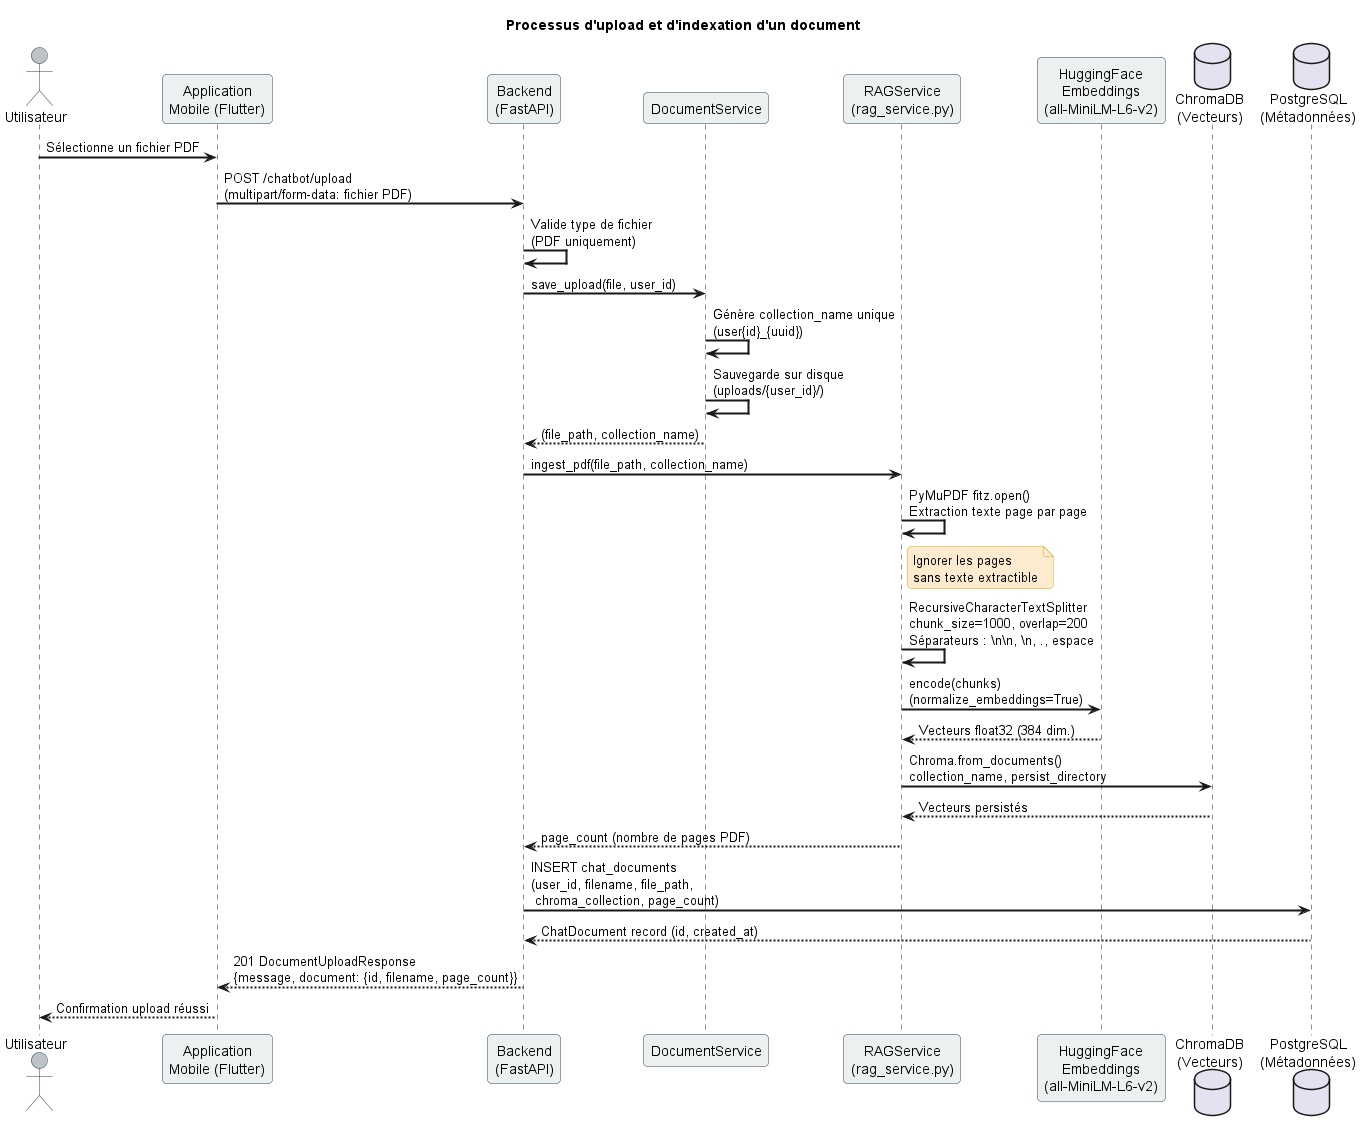
\includegraphics[width=0.85\textwidth]{images/seq_upload.jpg}
\caption{Diagramme de séquence du processus d'upload et d'indexation}
\label{fig:seq_upload}
\end{figure}

%----------------------------------------
\subsubsection{Processus de chat RAG}

Le processus de chat RAG permet à l'utilisateur d'interroger ses documents de manière contextuelle. Comme montré dans la Figure~\ref{fig:seq_chat_rag}, la question est envoyée au backend qui effectue une recherche sémantique dans ChromaDB. Les chunks les plus pertinents sont assemblés en contexte et envoyés à Gemini pour générer une réponse précise accompagnée de citations.

\begin{figure}[H]
\centering
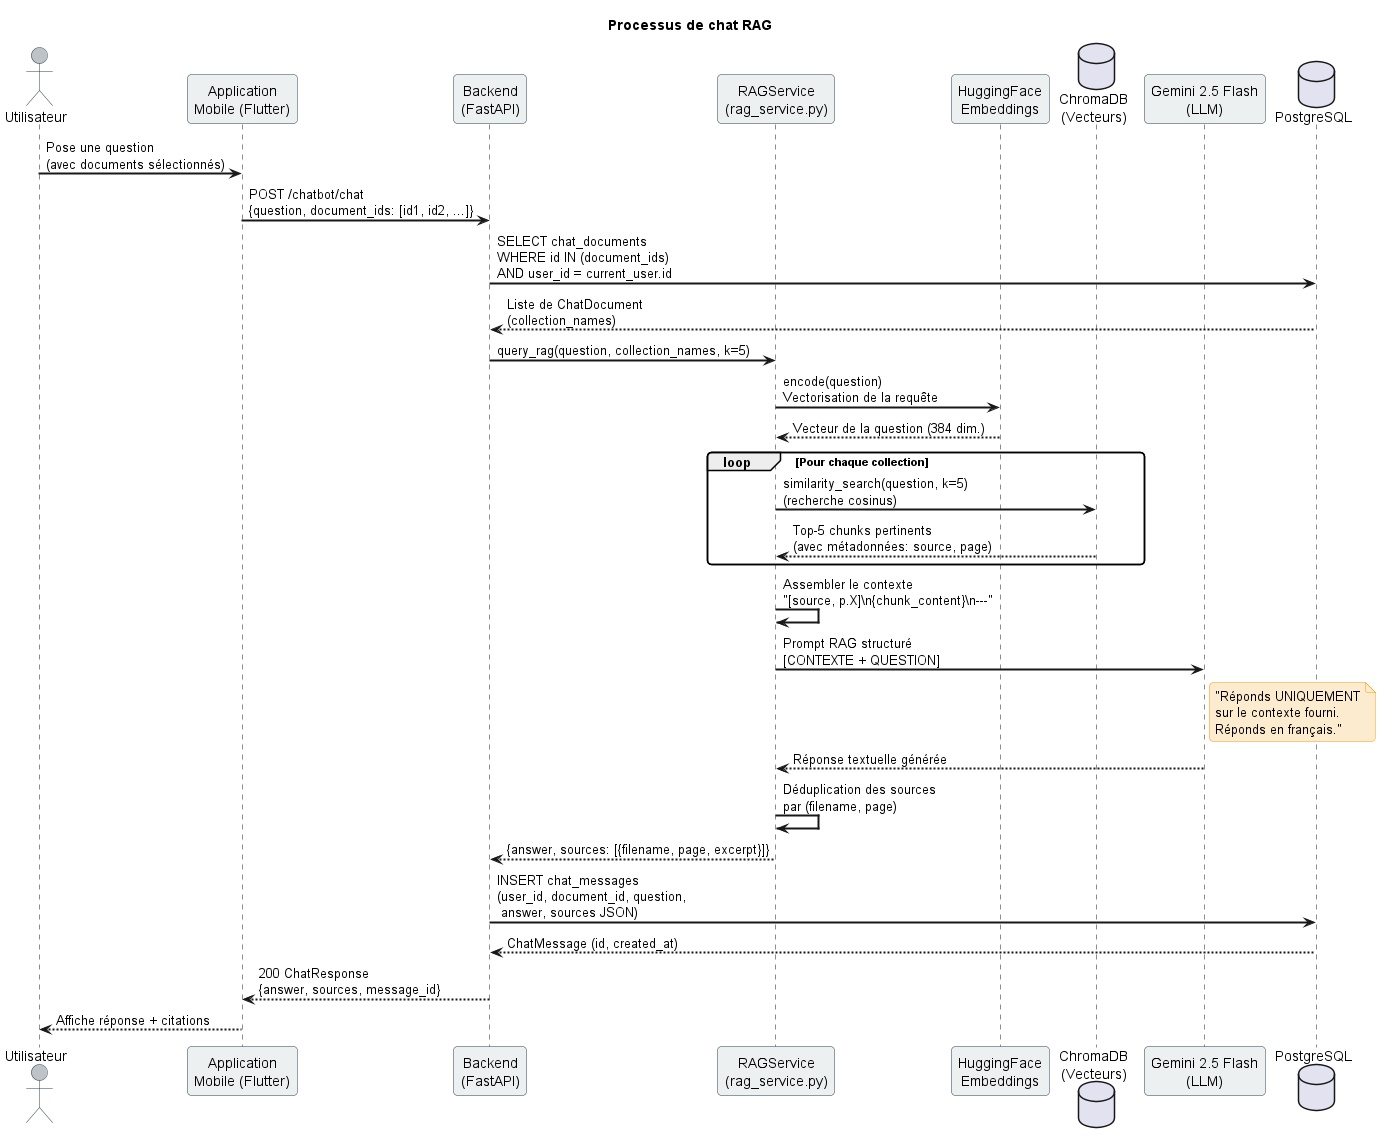
\includegraphics[width=0.85\textwidth]{images/seq_chat_rag.jpg}
\caption{Diagramme de séquence du processus de chat RAG}
\label{fig:seq_chat_rag}
\end{figure}

%----------------------------------------
\subsubsection{Processus de génération de quiz}

Le processus de génération de quiz exploite le contenu des documents indexés pour produire des questions à choix multiples. Comme illustré dans la Figure~\ref{fig:seq_quiz}, le backend récupère un échantillon diversifié de chunks, construit un prompt spécialisé et envoie la requête à Gemini. Le résultat JSON est validé avant d'être persisté en base de données.

\begin{figure}[H]
\centering
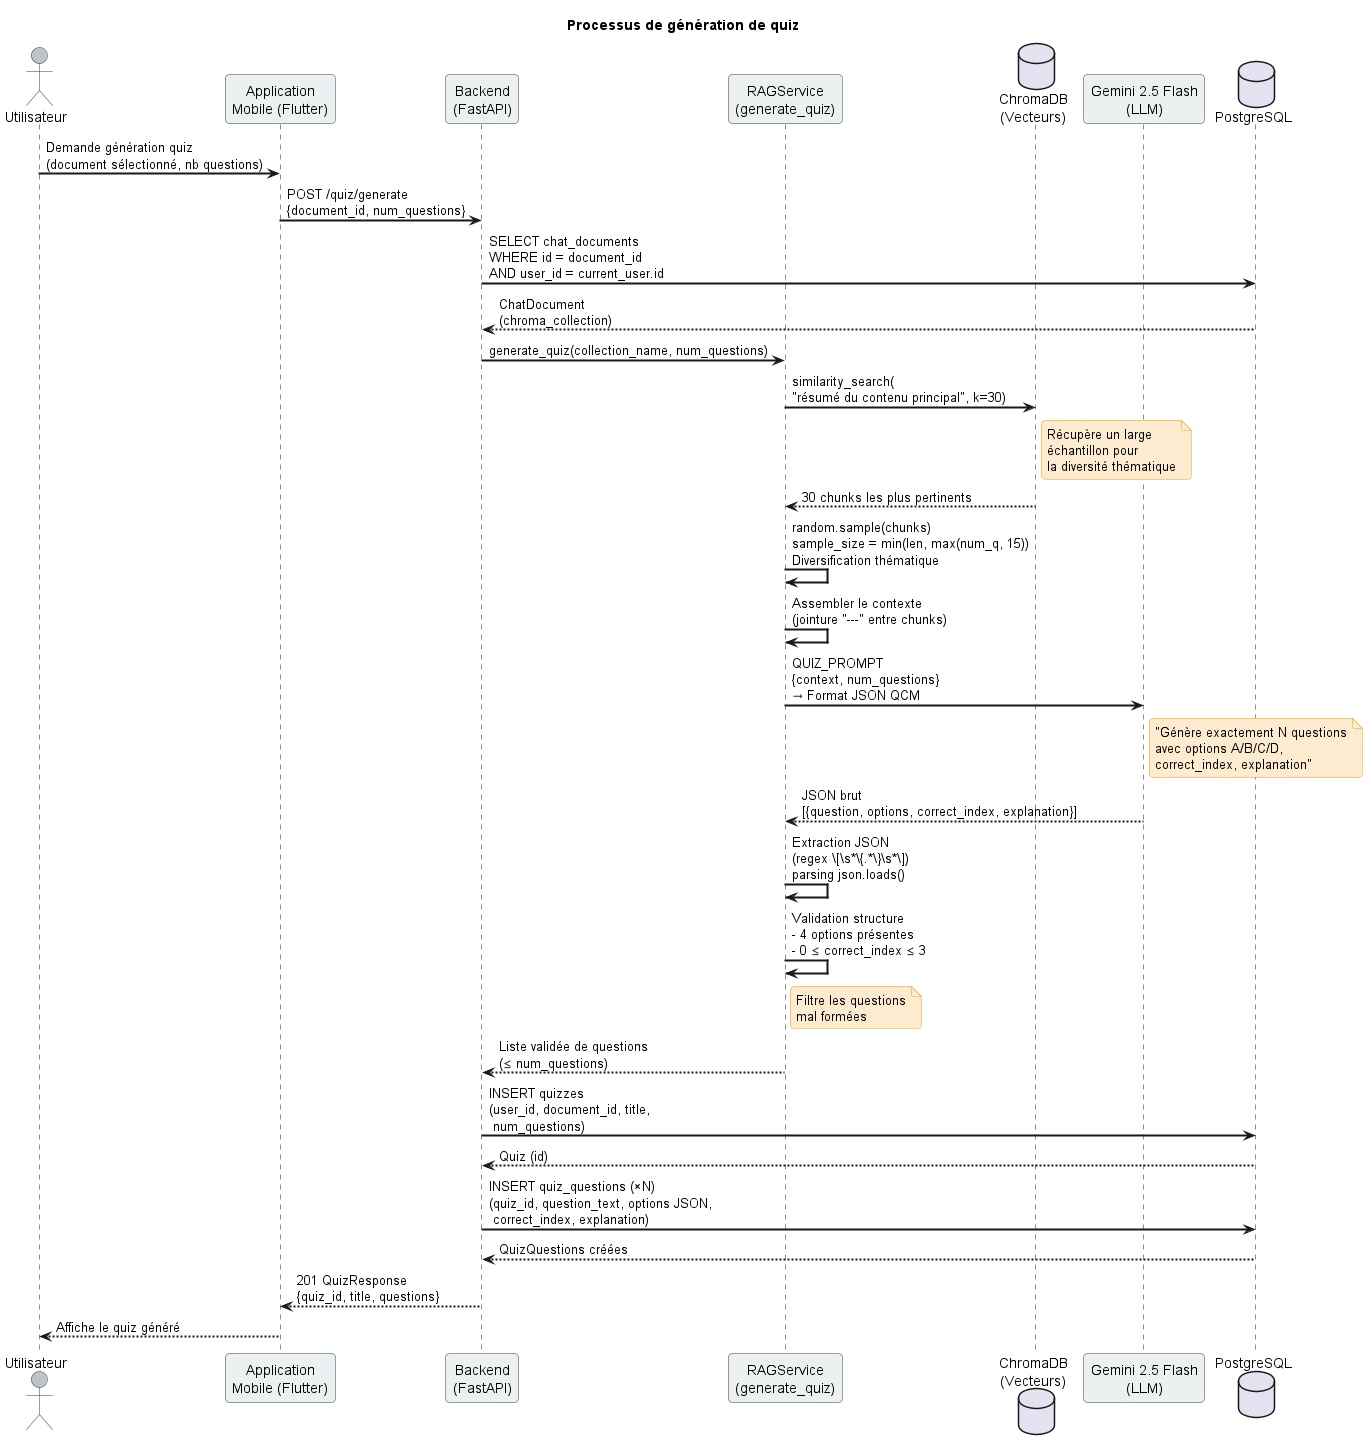
\includegraphics[width=0.85\textwidth]{images/seq_quiz.jpg}
\caption{Diagramme de séquence de la génération de quiz}
\label{fig:seq_quiz}
\end{figure}

%----------------------------------------
\subsubsection{Processus de génération du planning intelligent}

Le processus de planification combine un calcul algorithmique avec l'intelligence artificielle. Comme illustré dans la Figure~\ref{fig:seq_planning}, le backend détermine d'abord les créneaux libres de manière déterministe, puis demande à Gemini d'assigner des sujets pertinents à chaque créneau. En cas d'échec de l'IA, un mécanisme de fallback garantit la production d'un planning valide.

\begin{figure}[H]
\centering
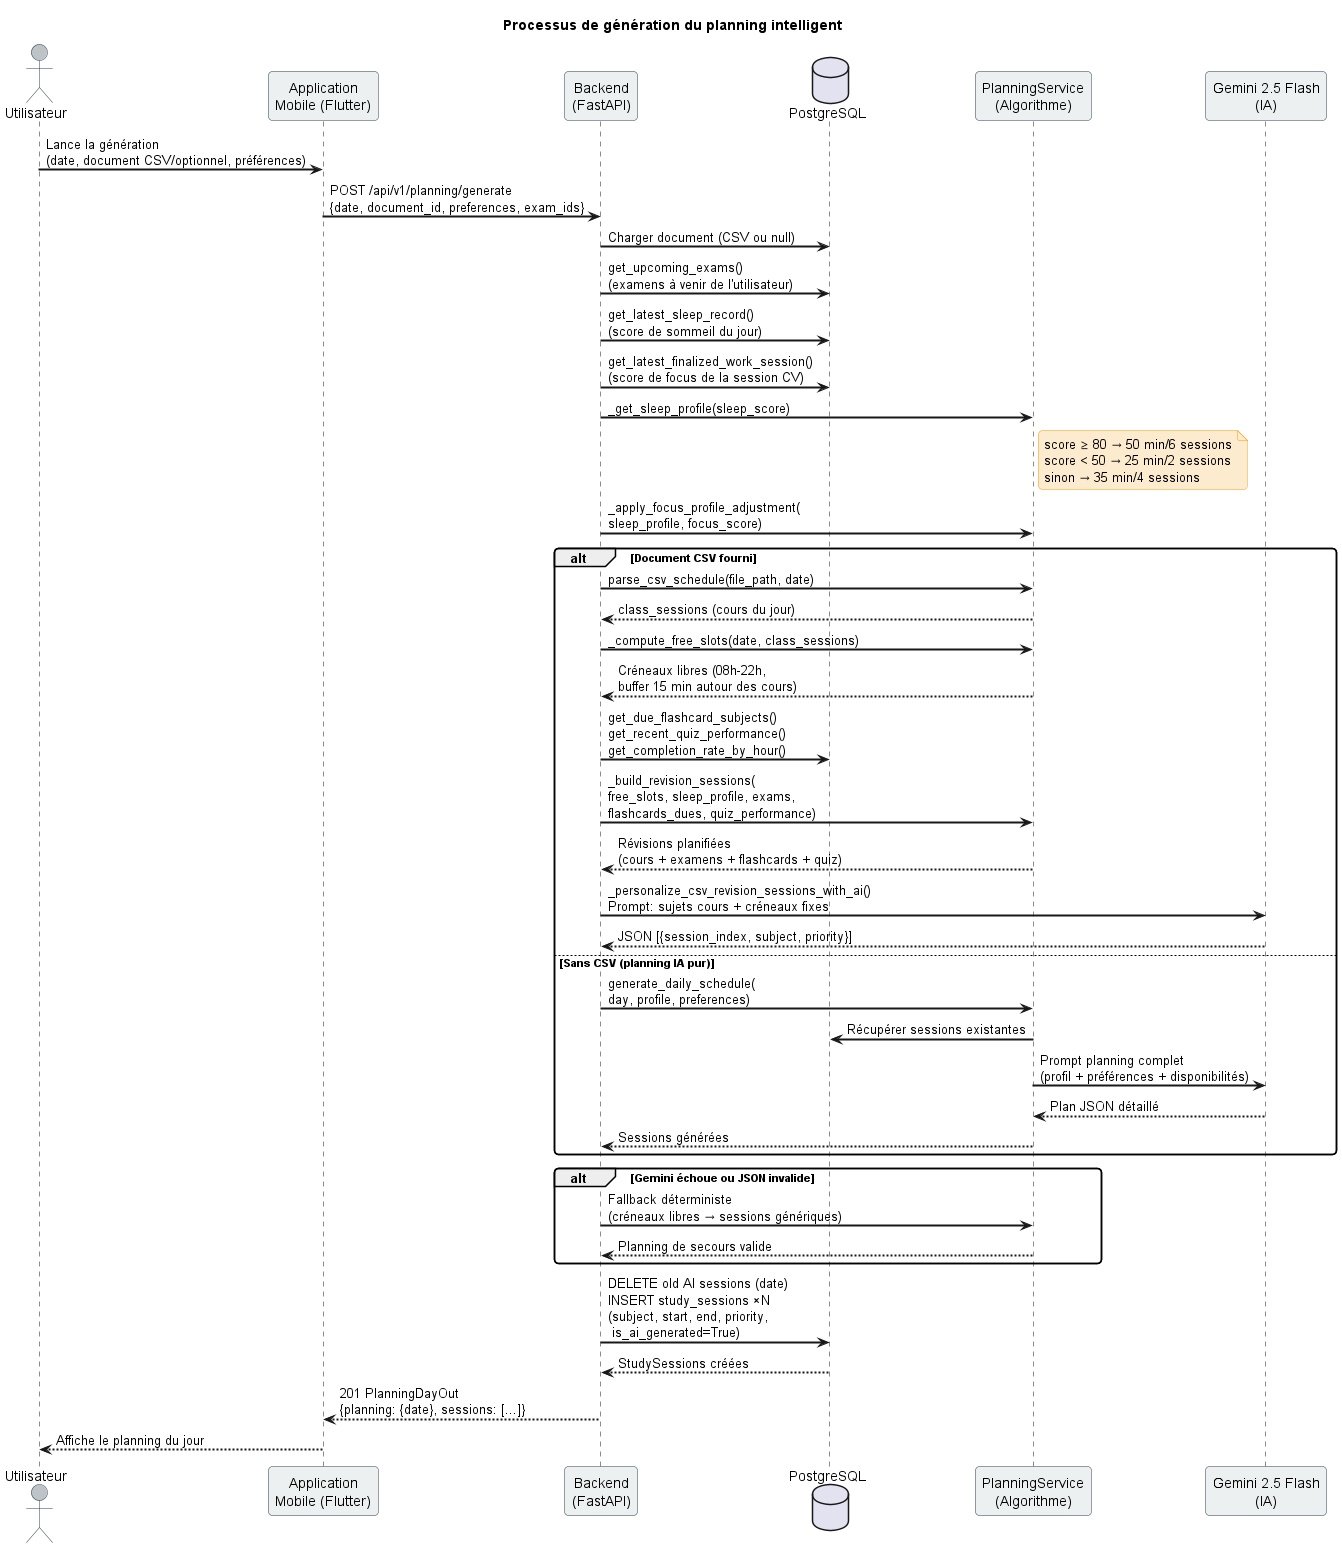
\includegraphics[width=0.85\textwidth]{images/seq_planning.jpg}
\caption{Diagramme de séquence de la génération du planning intelligent}
\label{fig:seq_planning}
\end{figure}


\subsection{Diagramme de classes du Sprint 3}

Le diagramme de classes présenté dans la Figure~\ref{fig:class_sprint3} décrit la structure des modules développés durant ce sprint.

La classe \textit{ChatDocument} représente un document importé et est associée aux messages du chatbot (\textit{ChatMessage}), aux quiz (\textit{Quiz}) et aux flashcards (\textit{Flashcard}). La classe \textit{Quiz} contient une liste de \textit{QuizQuestion}, chacune disposant d'options et d'une correction.

La classe \textit{Flashcard} intègre les paramètres de l'algorithme SM-2 (ease\_factor, interval, repetitions, next\_review). La classe \textit{StudySession} représente une session de planning avec son sujet, ses horaires et son statut.

Les services \textit{RAGService}, \textit{PlanningService} et \textit{SM2Service} centralisent respectivement les opérations de recherche sémantique, de planification et de répétition espacée.

\begin{figure}[H]
\centering
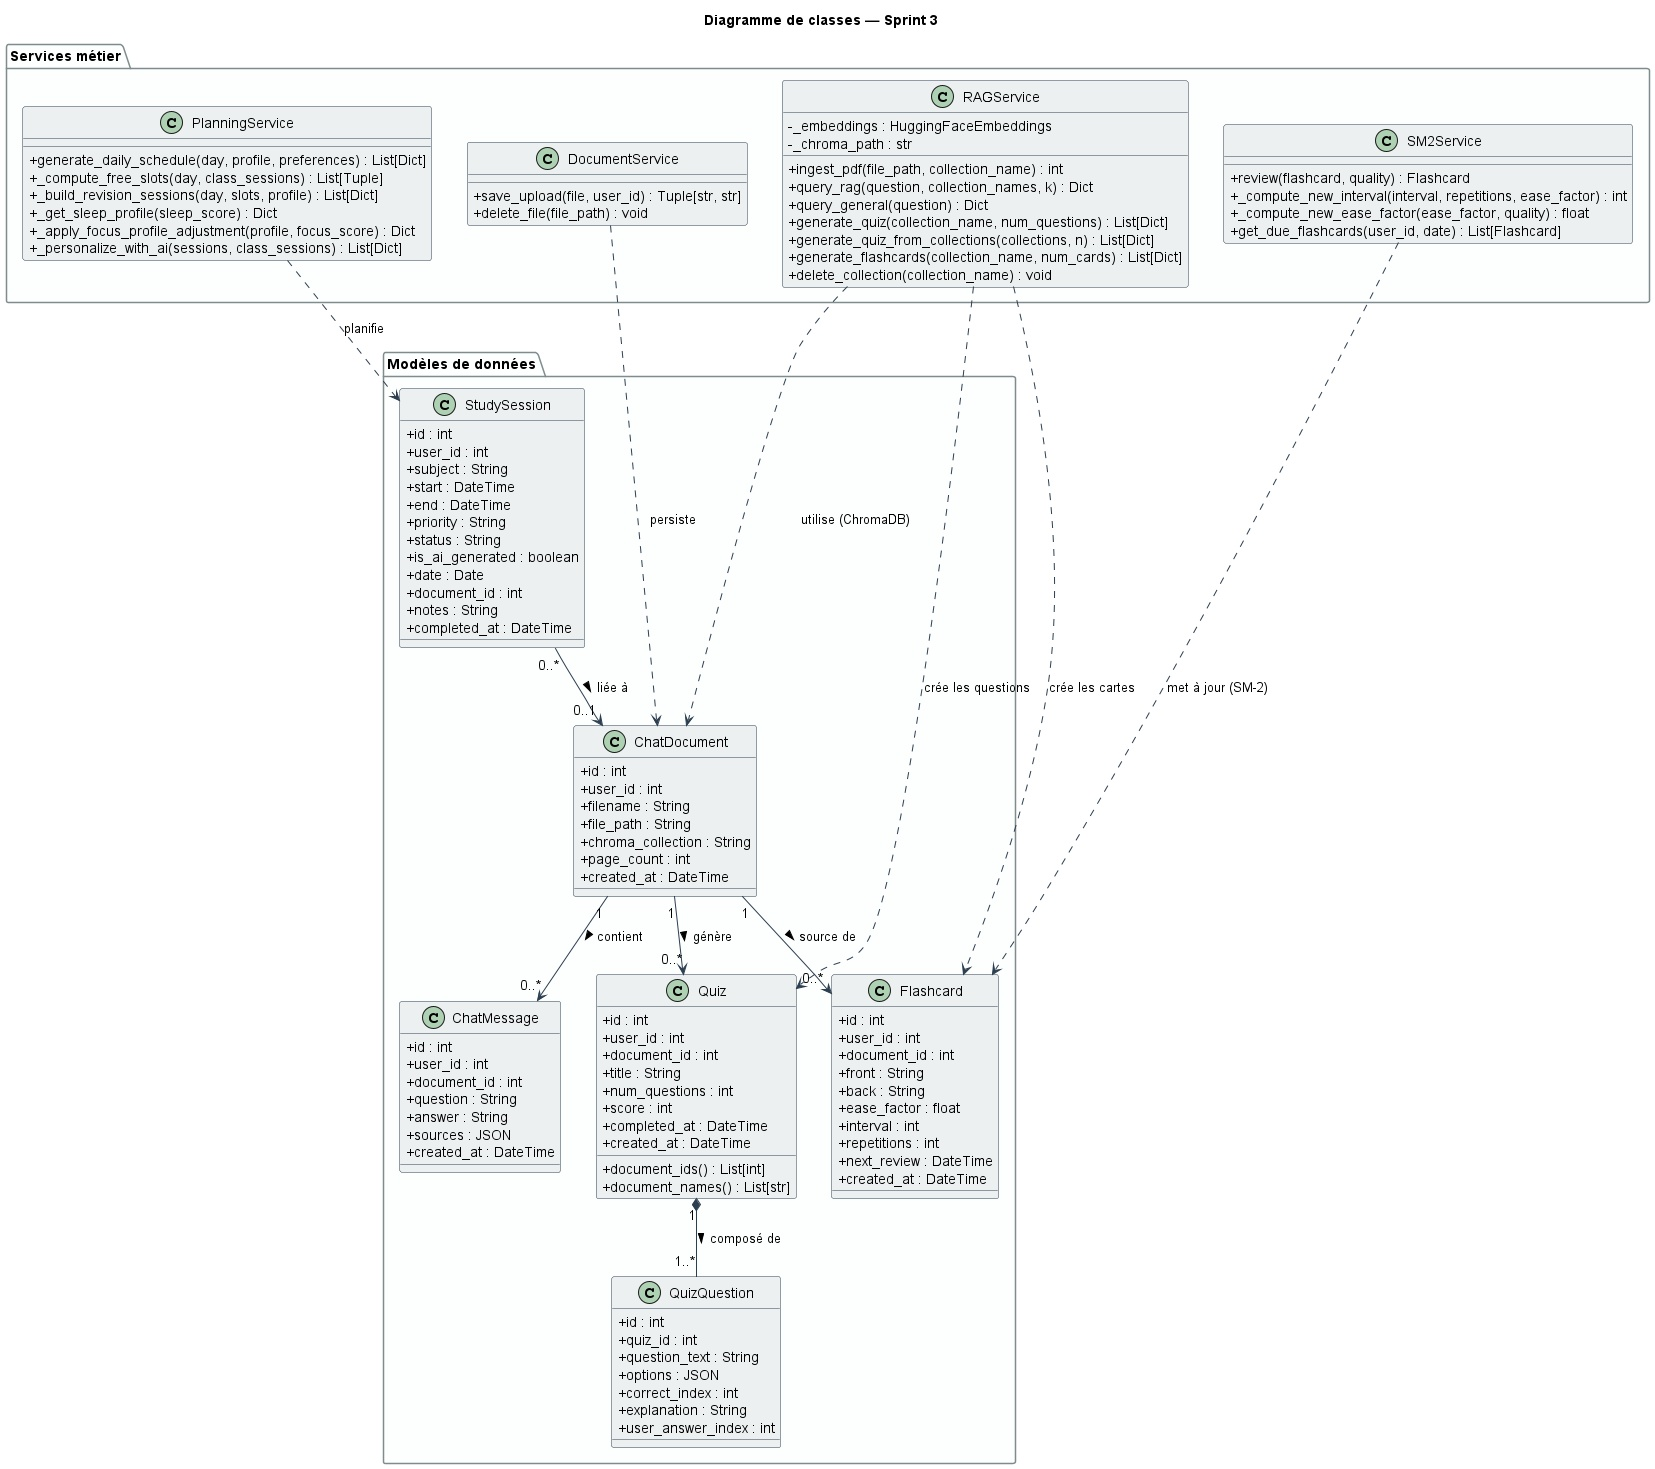
\includegraphics[width=0.85\textwidth]{images/class_sprint3.jpg}
\caption{Diagramme de classes du Sprint 3}
\label{fig:class_sprint3}
\end{figure}

%%%%%%%%%%%%%%%%%%%%%%%%%%%%%%%%%%%%%%%%%%%%%%%%%%%%%%%%%%%%%%%%
\section{Implémentation}

Cette section présente les principales interfaces développées dans le cadre du Sprint 3. Elles illustrent les fonctionnalités liées au chatbot RAG, à la génération de quiz et de flashcards, ainsi qu'à la planification intelligente.

%--------------------------------------

\subsection{Interfaces de l'application mobile}

Les interfaces développées dans le cadre du Sprint 3 permettent à l'utilisateur d'interagir avec les modules d'intelligence artificielle du système. Elles couvrent l'assistant pédagogique, les outils de révision et le planning adaptatif.

%----------------------------------------
\subsubsection{Interface du chatbot RAG}

L'interface du chatbot permet à l'utilisateur de poser des questions sur ses documents importés et d'obtenir des réponses contextualisées. Elle offre également la possibilité de sélectionner les documents sources et de consulter l'historique des échanges.

\begin{figure}[H]
\centering
\includegraphics[width=0.35\textwidth]{images/chatbot1.jpg}
\hspace{0.5cm}
\includegraphics[width=0.35\textwidth]{images/chatbot2.jpg}
\caption{Interface du chatbot RAG : gestion des documents et conversation}
\label{fig:chatbot_screens}
\end{figure}

%----------------------------------------
\subsubsection{Interfaces de génération et passage de quiz}

Ces interfaces permettent à l'utilisateur de générer des quiz QCM à partir de ses documents, de répondre aux questions et de consulter les résultats détaillés avec explications.

\begin{figure}[H]
\centering
\includegraphics[width=0.35\textwidth]{images/quiz1.jpg}
\hspace{0.5cm}
\includegraphics[width=0.35\textwidth]{images/quiz2.jpg}
\caption{Interfaces de quiz : génération et passage du quiz}
\label{fig:quiz_screens}
\end{figure}

%----------------------------------------
\subsubsection{Interfaces des flashcards avec révision espacée}

Les interfaces de flashcards permettent à l'utilisateur de générer des cartes de révision, de les parcourir et d'évaluer sa qualité de rappel. Le système utilise l'algorithme SM-2 pour planifier automatiquement les prochaines sessions de révision.

\begin{figure}[H]
\centering
\includegraphics[width=0.35\textwidth]{images/flashcard1.jpg}
\hspace{0.5cm}
\includegraphics[width=0.35\textwidth]{images/flashcard2.jpg}
\caption{Interfaces des flashcards : génération et révision}
\label{fig:flashcard_screens}
\end{figure}

%----------------------------------------
\subsubsection{Interface du planning intelligent}

L'interface de planning affiche les sessions d'étude générées automatiquement par le système. L'utilisateur peut consulter son planning quotidien ou hebdomadaire, créer des sessions manuellement, et visualiser l'adaptation des créneaux en fonction de son état de sommeil et de ses examens.

\begin{figure}[H]
\centering
\includegraphics[width=0.35\textwidth]{images/planning1.jpg}
\hspace{0.5cm}
\includegraphics[width=0.35\textwidth]{images/planning2.jpg}
\caption{Interface du planning intelligent : vue quotidienne et génération IA}
\label{fig:planning_screens}
\end{figure}

%%%%%%%%%%%%%%%%%%%%%%%%%%%%%%%%%%%%%%%%%%%%%%%%%%%%%%%%%%%%%%%

\section{Conclusion}
\addcontentsline{toc}{section}{Conclusion}

Ce troisième sprint a permis de mettre en place les modules d'intelligence artificielle au cœur du système \textit{Smart Focus}. Le chatbot RAG, les quiz QCM, les flashcards avec révision espacée SM-2 et le planning intelligent constituent désormais un ensemble cohérent d'outils pédagogiques.

L'architecture adoptée, combinant un calcul déterministe des créneaux avec une personnalisation par IA, garantit à la fois la fiabilité et la pertinence des résultats produits. Ces fonctionnalités posent les bases pour l'intégration du monitoring temps réel et des alertes intelligentes dans le sprint suivant.

